\documentclass[absolute, overlay]{TIBbeamer}

%%%% Usepackages

\usepackage[english]{babel}
\usepackage{color}
\usepackage{epstopdf}
\usepackage{graphicx}
\usepackage{hyperref}
\usepackage{tikz}
\usepackage{xcolor}

%%%% Miscellaneous Settings

\graphicspath{{graphics/}}

\defbeamertemplate{description item}{align left}{\insertdescriptionitem\hfill}

\AtBeginSection{\frame{\sectionpage}}

%%%% Title Page

\title{Fachinformation Informatik / Mathematik}

\author{Mila Runnwerth}

\date{F�r das Team Zentrale Information, 11. \& 18. Februar 2016}

\begin{document}

%%%%%%%%%%%%%%%%%%%%%%%%%%%%%%%%%%%%%

\begin{frame}
\titlepage
\end{frame}

%%%%%%%%%%%%%%%%%%%%%%%%%%%%%%%%%%%%%

\begin{frame}{Inhalts\"ubersicht}
\thispagestyle{empty}
\tableofcontents
\end{frame}

%%%%%%%%%%%%%%%%%%%%%%%%%%%%%%%%%%%%%

\section{Lern- und Arbeitsverhalten}

\subsection{Wissenschaftliches Arbeiten}

%%%%%%%%%%%%%%%%%%%%%%%%%%%%%%%%%%%%%

\begin{frame}{Wissenschaftliches Arbeiten (1/2)}

\centering
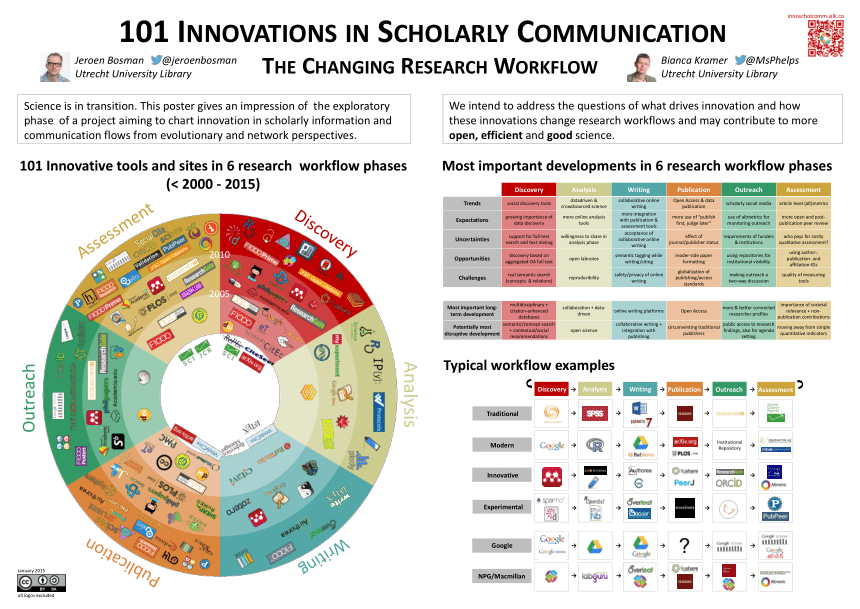
\includegraphics[width=0.75\linewidth]{101innovations} \\
\tiny{\href{https://s3-eu-west-1.amazonaws.com/pfigshare-u-previews/1863601/page_1_width_860.png}{Bosman, Kramer: 101 Innovations in Scholarly Communication}}

\end{frame}

%%%%%%%%%%%%%%%%%%%%%%%%%%%%%%%%%%%%%

\begin{frame}{Wissenschaftliches Arbeiten (2/2)}

\end{frame}

%%%%%%%%%%%%%%%%%%%%%%%%%%%%%%%%%%%%%

\begin{frame}{Dann kann es los gehen.}

\begin{figure}
\begin{minipage}{0.59\linewidth}
\flushleft
Nun betrachten wir die Werkzeugkasten, die in der Mathematik und in der Informatik jeweils in den entsprechenden Phasen zur Verf\"ugung stehen.
\end{minipage}
\begin{minipage}{0.4\linewidth}
\centering
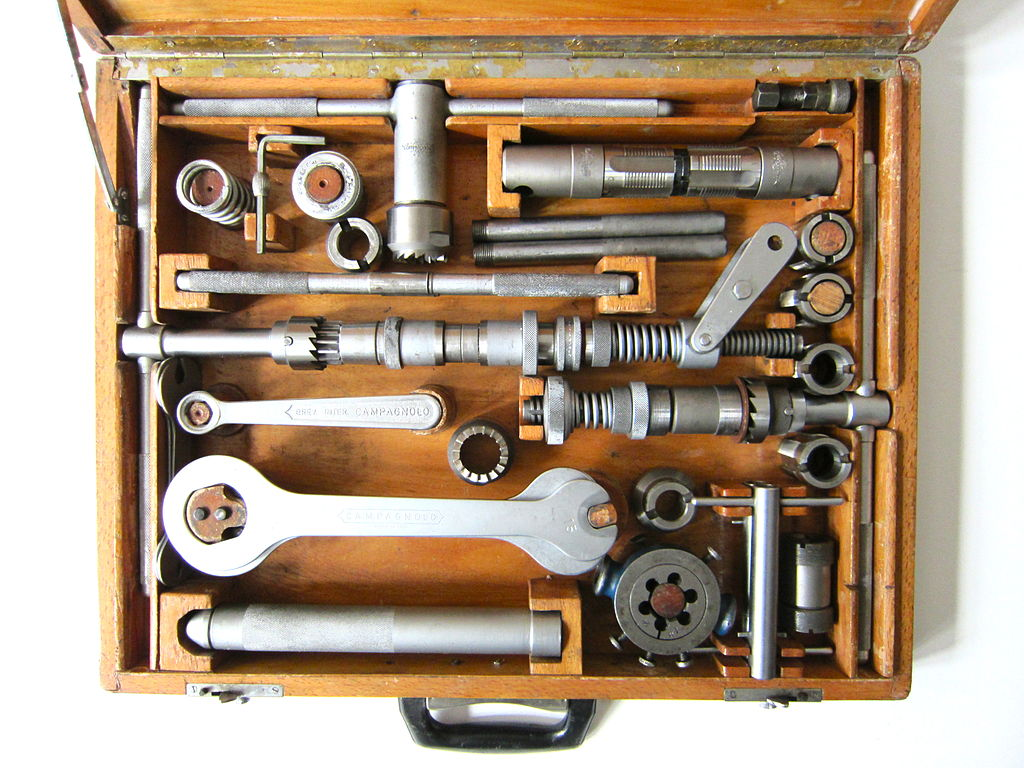
\includegraphics[width=0.8\linewidth]{toolbox} \\
\tiny{\href{https://upload.wikimedia.org/wikipedia/commons/thumb/3/3f/Campagnolo_1968_Tool_Kit_Wooden_Box.jpg/1024px-Campagnolo_1968_Tool_Kit_Wooden_Box.jpg}{Wikipedia}}
\end{minipage}
\end{figure}

\end{frame}

%%%%%%%%%%%%%%%%%%%%%%%%%%%%%%%%%%%%%

\section{Informatik}

%%%%%%%%%%%%%%%%%%%%%%%%%%%%%%%%%%%%%

\begin{frame}{Tja}

\end{frame}

%%%%%%%%%%%%%%%%%%%%%%%%%%%%%%%%%%%%%

\section{Mathematik}

%%%%%%%%%%%%%%%%%%%%%%%%%%%%%%%%%%%%%

\section{Fachinformationsdienst Mathematik}

%%%%%%%%%%%%%%%%%%%%%%%%%%%%%%%%%%%%%

\section{Anregungen \& Fragen}

%%%%%%%%%%%%%%%%%%%%%%%%%%%%%%%%%%%%%

\begin{frame}{Anregungen \& Fragen}

\end{frame}

%%%%%%%%%%%%%%%%%%%%%%%%%%%%%%%%%%%%%

\end{document}
